% En los listados, los dos puntos, paréntesis y operadores con guion son
% sintaxis de SystemVerilog; los rangos y referencias también usan guiones.
% chktex-file 1
% chktex-file 8
% chktex-file 13
% chktex-file 26
% chktex-file 36

\section{Contrato del núcleo}

Una vez separada la interfaz de la placa, el contrato de la ALU
resulta pequeño: recibe dos operandos y un código de operación, y
entrega un resultado acompañado por tres indicadores. Los operandos y
la salida comparten el ancho \texttt{NB\_DATA}; el control utiliza
\texttt{NB\_OPCODE} bits. En la implementación utilizada para la
\tech{Basys 3} esos parámetros toman los valores 8 y 6, respectivamente.

Esta interfaz permite analizar el núcleo como una función
combinacional. No existen registros internos ni señales de
habilitación: cualquier cambio en A, B u opcode produce un nuevo
resultado después del retardo de propagación de la lógica.

\section{Operaciones implementadas}

Los códigos elegidos y su comportamiento se resumen en la
tabla~\ref{tab:operaciones}. En las operaciones booleanas se aplica
la función correspondiente a cada par de bits. En los
desplazamientos, B representa la cantidad de posiciones que debe desplazarse A.

\begin{table}[H]
  \centering
  \begin{tabularx}{\textwidth}{L{2.0cm}C{2.2cm}L{3.3cm}Y}
    \toprule
    \textbf{Operación} & \textbf{Opcode} & \textbf{Expresión} &
    \textbf{Descripción} \\
    \midrule
    ADD & \texttt{100000} & \texttt{A + B} & Suma \\
    SUB & \texttt{100010} & \texttt{A - B} & Resta \\
    AND & \texttt{100100} & \texttt{A \& B} & AND bit a bit \\
    OR  & \texttt{100101} & \texttt{A | B} & OR bit a bit \\
    XOR & \texttt{100110} & \texttt{A \string^ B} & XOR bit a bit \\
    SRA & \texttt{000011} & \texttt{\$signed(A) >>> B} &
    Desplazamiento aritmético a derecha \\
    SRL & \texttt{000010} & \texttt{A >> B} & Desplazamiento lógico a derecha \\
    NOR & \texttt{100111} & \texttt{\string~(A | B)} & NOR bit a bit \\
    \bottomrule
  \end{tabularx}
  \caption{Operaciones implementadas por la ALU.}%
  \label{tab:operaciones}
\end{table}

La diferencia entre los dos desplazamientos se vuelve visible cuando
el bit más significativo de A vale uno. Si A es \texttt{80} y B es
\texttt{01}, \tech{SRL} introduce un cero por la izquierda y produce
\texttt{40}. Por el contrario, \tech{SRA} interpreta A con signo y replica
ese uno, por lo que obtiene \texttt{C0}.

Los códigos que no aparecen en la tabla producen cero. No se trata de
una operación adicional, sino de una decisión defensiva: todas las
combinaciones de la entrada quedan definidas y el circuito nunca
necesita conservar el resultado anterior.

\section{Interpretación de los indicadores}

Con ocho bits, un mismo patrón puede representar un valor entre
\num{0} y \num{255} sin signo o uno entre \num{-128} y \num{127} en
complemento a dos. Carry y
overflow describen desbordamientos diferentes; por eso no deben
interpretarse como indicadores equivalentes. La
tabla~\ref{tab:indicadores} resume la condición de activación de cada
salida.

\begin{table}[H]
  \centering
  \begin{tabularx}{\textwidth}{L{2.7cm}L{3.2cm}Y}
    \toprule
    \textbf{Salida} & \textbf{Indicador} & \textbf{Condición} \\
    \midrule
    \texttt{o\_zero} & Cero, Z & Todos los bits del resultado son cero. \\
    \texttt{o\_carry} & Acarreo, C & ADD genera un bit adicional
    fuera del ancho de la salida. \\
    \texttt{o\_overflow} & Desbordamiento, V & ADD o SUB excede el
    rango representable con signo. \\
    \bottomrule
  \end{tabularx}
  \caption{Indicadores generados por el núcleo.}%
  \label{tab:indicadores}
\end{table}

El caso \texttt{FF + 01} muestra el carry. Interpretados sin signo,
los operandos valen \num{255} y \num{1}; el resultado completo es
\num{256} y necesita
nueve bits. La salida conserva \texttt{00}, Z se activa porque esos
ocho bits son cero y C conserva el bit adicional. En complemento a
dos, en cambio, la misma entrada representa $-1+1=0$, por lo que V
permanece apagado.

La suma \texttt{7F + 01} presenta la situación inversa. El valor \num{128}
cabe en ocho bits sin signo y no genera carry, pero supera el máximo
positivo en complemento a dos. La salida \texttt{80} se interpretaría
como \num{-128}; V advierte que ese patrón ya no representa la suma con
signo esperada.

La misma regla alcanza la resta. En \texttt{80 - 01}, el resultado
matemático con signo es \num{-129}, que queda fuera del rango. Los ocho
bits conservados forman \texttt{7F} y V se activa. C permanece en
cero porque en este trabajo no se utiliza como indicador de préstamo.

\begin{table}[H]
  \centering
  \begin{tabular}{ccccccc}
    \toprule
    \textbf{A} & \textbf{B} & \textbf{Operación} & \textbf{Resultado}
    & \textbf{Z} & \textbf{C} & \textbf{V} \\
    \midrule
    \texttt{05} & \texttt{03} & ADD & \texttt{08} & 0 & 0 & 0 \\
    \texttt{FF} & \texttt{01} & ADD & \texttt{00} & 1 & 1 & 0 \\
    \texttt{7F} & \texttt{01} & ADD & \texttt{80} & 0 & 0 & 1 \\
    \texttt{80} & \texttt{80} & ADD & \texttt{00} & 1 & 1 & 1 \\
    \texttt{80} & \texttt{01} & SUB & \texttt{7F} & 0 & 0 & 1 \\
    \texttt{7F} & \texttt{FF} & SUB & \texttt{80} & 0 & 0 & 1 \\
    \texttt{05} & \texttt{05} & SUB & \texttt{00} & 1 & 0 & 0 \\
    \bottomrule
  \end{tabular}
  \caption{Casos representativos para distinguir Z, C y V.}
\end{table}

\section{Descripción combinacional}

El núcleo se implementa con un bloque \texttt{always\_comb} y una
sentencia \texttt{case}. Carry y overflow reciben un valor
predeterminado antes de seleccionar la operación; ADD y SUB los
reemplazan cuando corresponde. El caso \texttt{default} asigna el
resultado nulo. Esta estructura garantiza que todas las salidas
tengan un valor en cada evaluación y evita inferir latches.

\begin{codebox}[language=SystemVerilog]
  always_comb begin
  o_carry = 1'b0;
  o_overflow = 1'b0;

  case (i_data_opcode)
  OP_ADD: begin
  {o_carry, o_result} =
  {1'b0, i_data_a} + {1'b0, i_data_b};
  o_overflow =
  (i_data_a[NB_DATA-1] == i_data_b[NB_DATA-1]) &&
  (o_result[NB_DATA-1] != i_data_a[NB_DATA-1]);
  end

  OP_SUB: begin
  o_result = i_data_a - i_data_b;
  o_overflow =
  (i_data_a[NB_DATA-1] != i_data_b[NB_DATA-1]) &&
  (o_result[NB_DATA-1] != i_data_a[NB_DATA-1]);
  end

  // Operaciones logicas y desplazamientos.
  default: o_result = {NB_DATA{1'b0}};
  endcase
  end
\end{codebox}

En ADD, la suma se amplía un bit para conservar el acarreo sin signo.
El overflow se obtiene comparando los signos de los operandos y de la
salida. SUB utiliza una condición análoga, pero parte de operandos
con signos distintos. Las operaciones restantes se expresan
directamente mediante los operadores de \tech{SystemVerilog};
\texttt{\$signed} permite que SRA replique el signo.

El indicador Z no depende de la operación elegida, sino únicamente
del patrón final. Por eso se calcula con una asignación común fuera del bloque:

\begin{codebox}[language=SystemVerilog]
  assign o_zero = (o_result == {NB_DATA{1'b0}});
\end{codebox}

La figura~\ref{fig:alu-rtl} permite cerrar el recorrido entre
descripción y circuito. A la izquierda aparecen las funciones
aritméticas, lógicas y de desplazamiento; sus salidas llegan a
multiplexores controlados por el opcode. A la derecha se reconoce la
lógica que selecciona los indicadores. El esquema no agrega una
arquitectura nueva: es la interpretación que \tech{Vivado} realiza
del contrato y de las expresiones anteriores.

\begin{figure}[H]
  \centering
  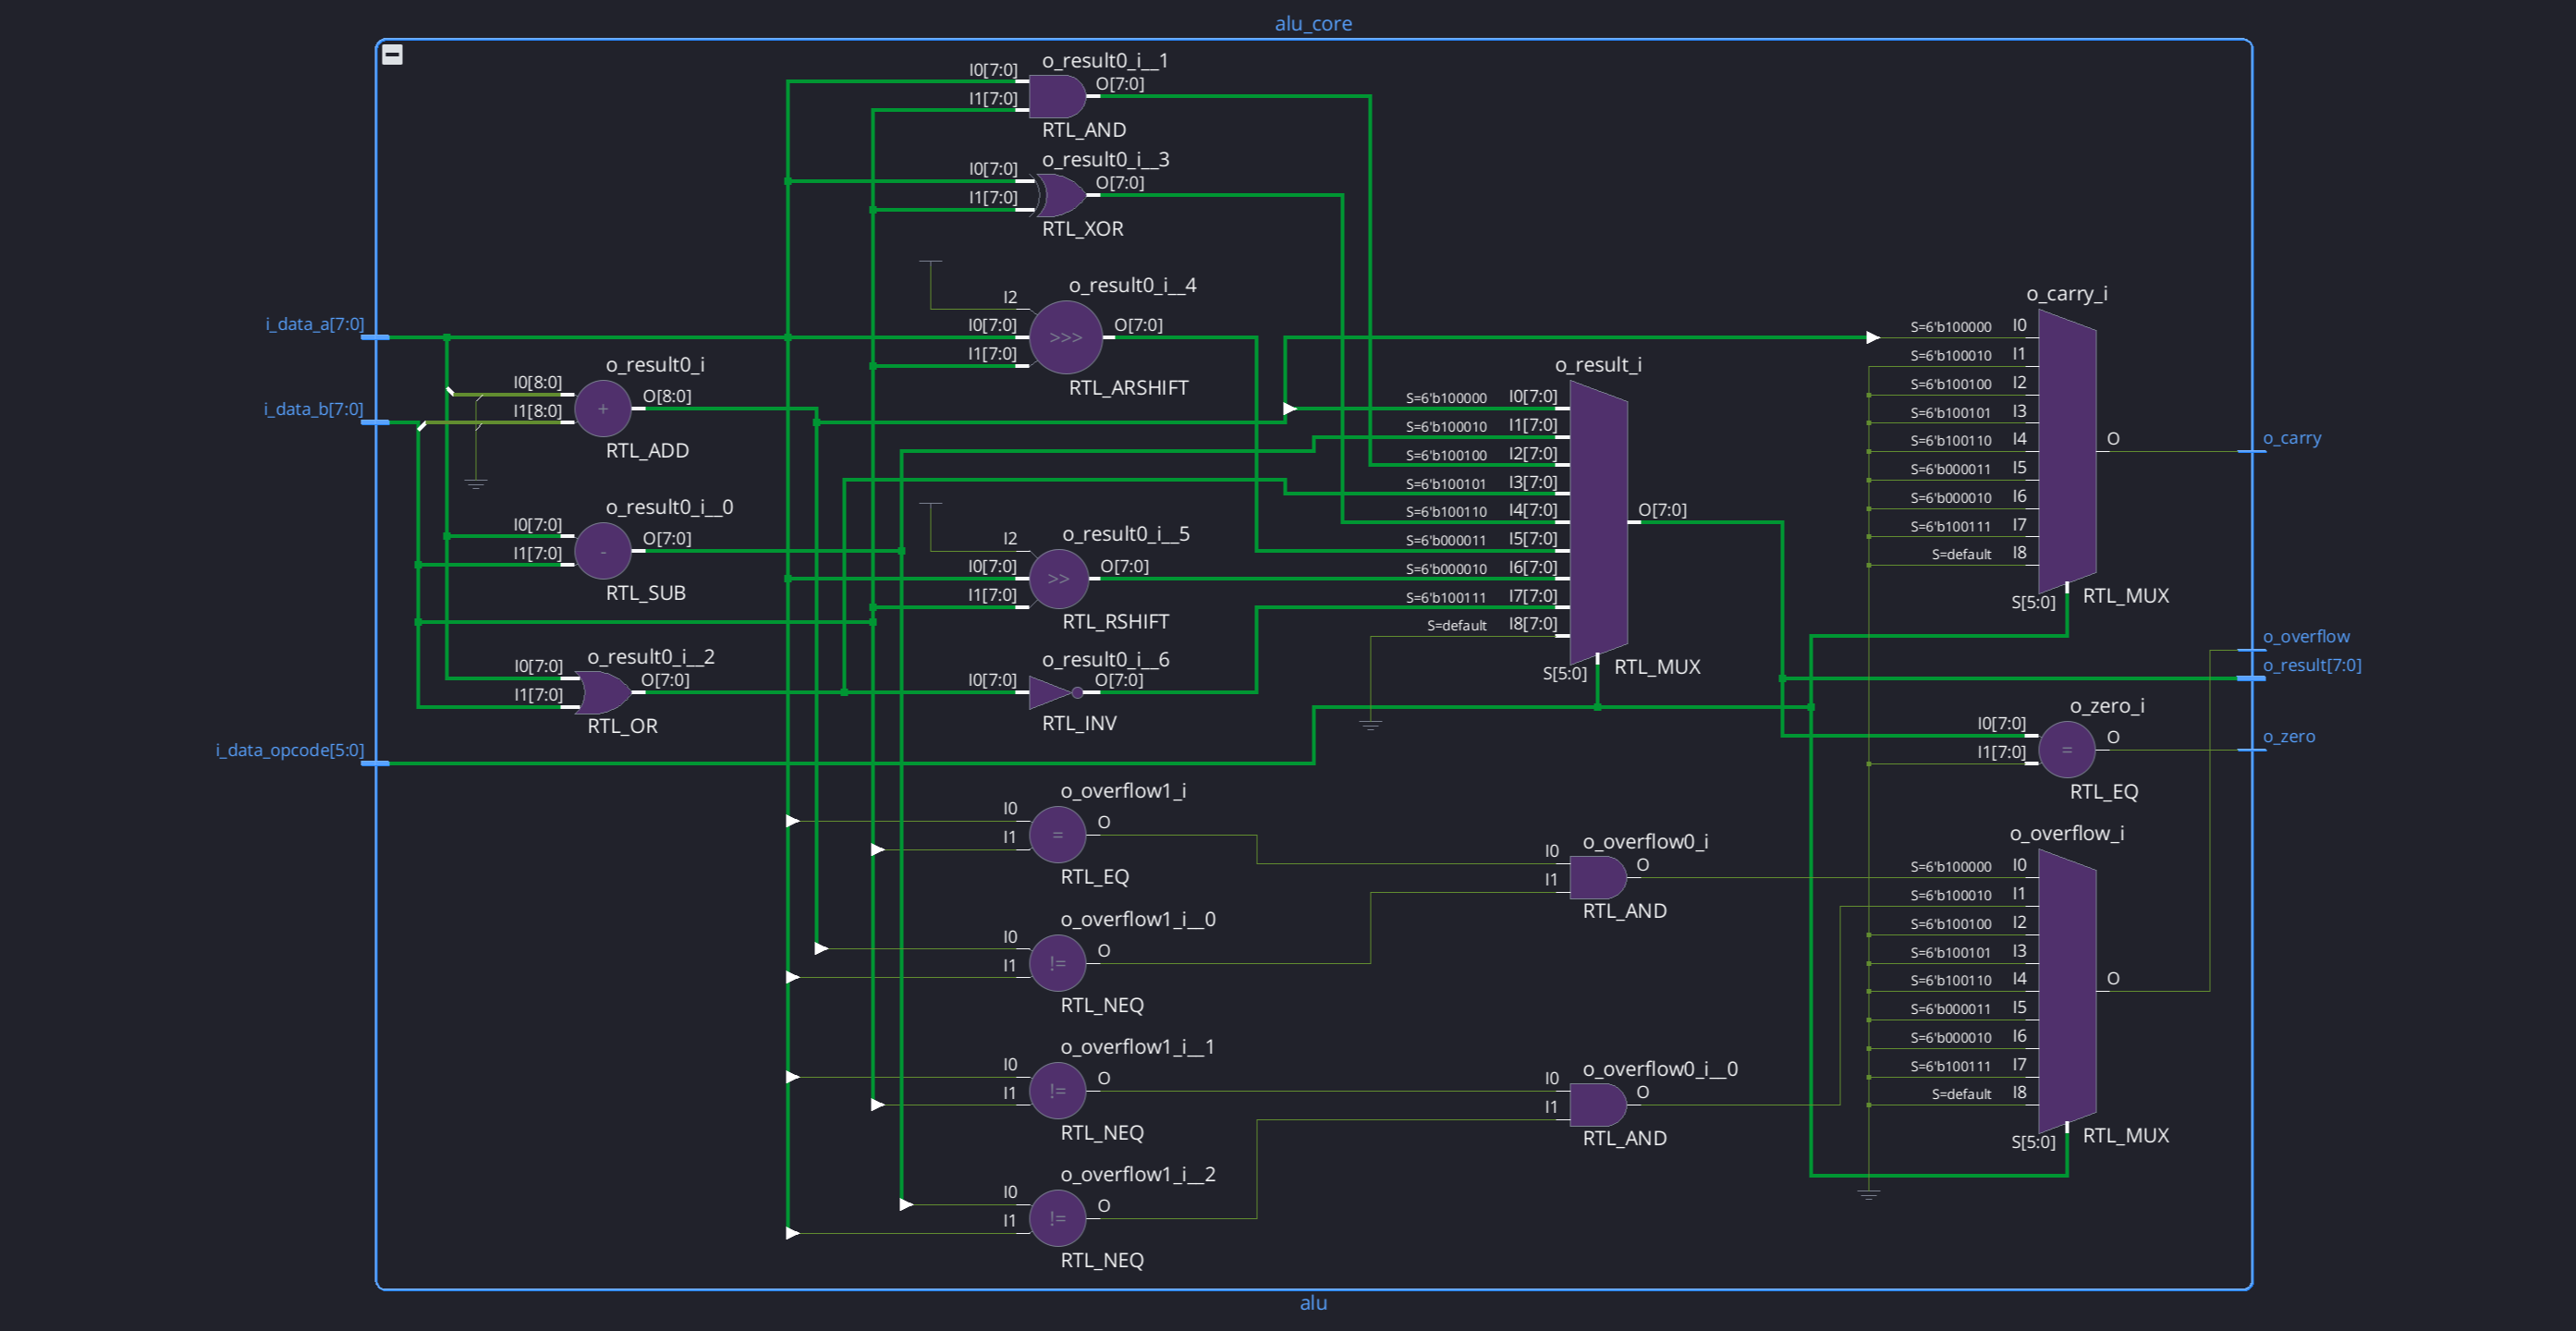
\includegraphics[width=\textwidth]{img/schematic_alu_rtl.png}
  \caption{Operaciones, selección del resultado e indicadores en la vista RTL.}%
  \label{fig:alu-rtl}
\end{figure}
